\subsection{Physics Engines}

\subsubsection{Open Dynamics Engine (ODE)}
\subsubsection{PhysX}


\subsection{Rendering Engines}  % Maybe not needed
\subsubsection{Open Graphics Rendering Engine (OGRE)}

\subsection{Game Engines}
The purpose of a game engine is to work as a fundamental back-end for most video games and simulators. A game engine is a software tool which allows interactive digital content to be made using a framework which easily allows the user to run it on different platforms such as computers, smartphones and consoles \cite{GameEngine_UnityGame_book}. Game engines are complex and consists of many components such as a physics engine, a rendering engine and other interactive tools to help the creator. They give the creator the freedom to control everything from lighting and audio to animation and character behavior in their game.
\\~\\
There exists many different game engines, but the two main ones that are currently in existence is Unity and Unreal Engine. These allow beginners to easily create their first games, as well as professional companies creating their games for millions of users \cite{GamesMadeInUnity, GamesMadeInUnrealEngine}.

\subsubsection{Unity}
Unity is currently the most commonly used game engine and over 2.5 million registered developers \cite{Unity_arnia_software}. Unity is developed by Unity Technologies and was first released June 2005.  Originally Unity was Over 60\% of augmented- and virtual reality games are created using Unity  \cite{GameEngine_UnityGame_book}. 
\\~\\
Unity is free for personal and educational projects. To create the game, Unity allows a lot of features using the GUI, but for full freedom the creator would need to program in C\#. Unity however provide lots of resources to learn C\#. Unity also combines with Visual Studio where the intellisense can help with recommending functions to use as well as spot errors\footnote{\url{https://docs.microsoft.com/en-us/visualstudio/gamedev/unity/get-started/getting-started-with-visual-studio-tools-for-unity}}.

\subsubsection{Unreal Engine}
Unreal Engine is a fast growing game engine and is created by Epic Games \cite{UnrealEngine_Book}. The first version of Unreal Engine was released in 1998, but Unreal Engine 4 (UE4), which was released September 2014, is their latest game engine. They have however announced that they will release Unreal Engine 5 (UE5) at the end of 2021 \cite{UE5}. 
\\~\\
UE4 has a variety of different use cases as well as games. TV broadcastes such as Sky Sports and BBC are using Unreal Engine for their graphical match analysis \cite{UnrealEngine_LiveBroadcast}. Professional architects are also using the product to illustrate their creations \cite{UnrealEngine_Automative}.   
\\~\\
Unreal Engine 4 is free for personal use and business making less than \$1 million in gross revenue \cite{UE5}. The code for UE4 is available on GitHub\footnote{\url{https://github.com/EpicGames/UnrealEngine}} (For access to the repository you would need to sign up for an Epic Games account\footnote{\url{https://www.unrealengine.com/en-US/ue4-on-github}}). UE4 allows two different ways for users to program their games. Either by using C++, which links with Visual Studio\footnote{\url{https://docs.unrealengine.com/en-US/ProductionPipelines/DevelopmentSetup/VisualStudioSetup/index.html}}, or by using blueprints as illustrated in Figure~\ref{UnrealEngineBlueprint}. Blueprints allows the creator for most of the freedom code gives them, but in an easier drag and drop layout.
\\~\\
The majority of the simulators that will be looked at later use Unreal Engine as their game engine. 

\begin{figure}[H] 
    \centering
    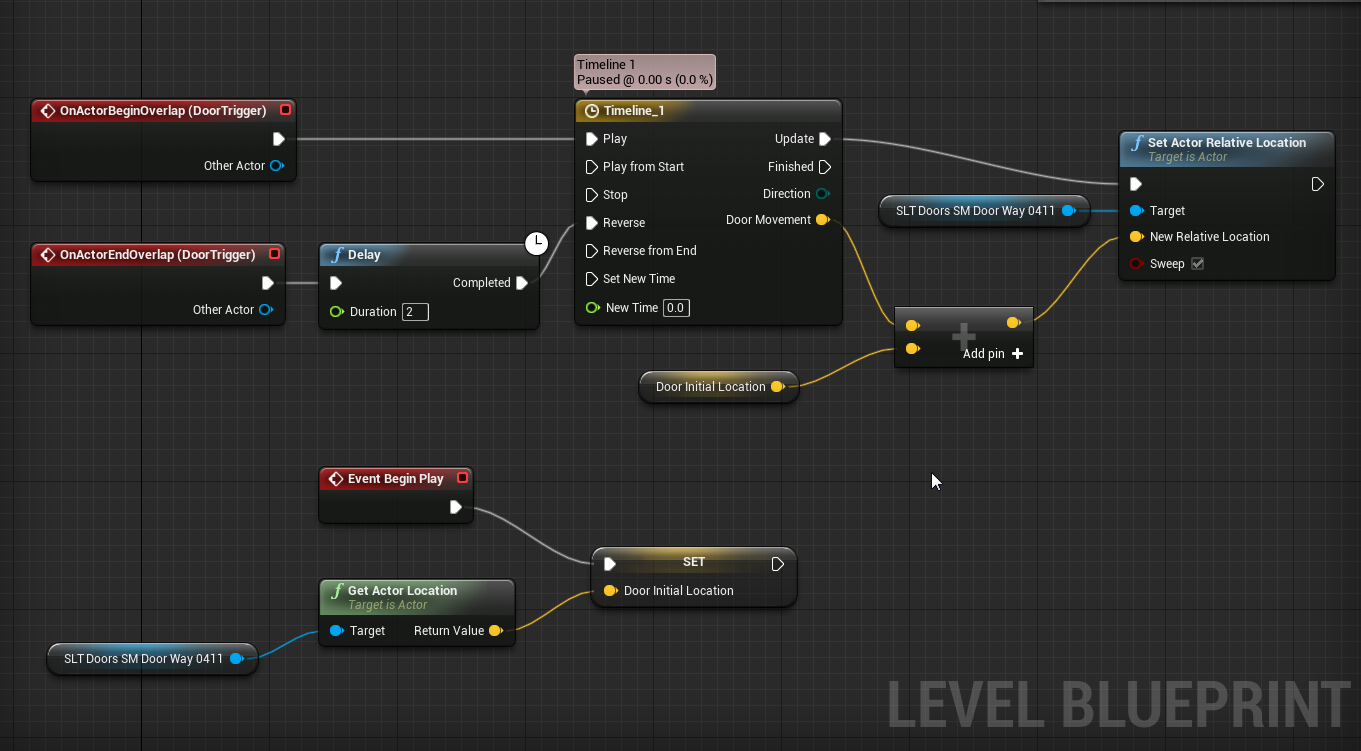
\includegraphics[width=0.5\textwidth]{OtherImages/UEBlueprint.png}
    \caption{Source: \url{https://docs.unrealengine.com/en-US/ProgrammingAndScripting/Blueprints/UserGuide/Timelines/Examples/OpeningDoors/index.html}}    \label{UnrealEngineBlueprint}

\end{figure}

\subsection{Vehicle Autonomy}
% 5 Levels
\subsection{Traffic Simulators}


\subsection{Machine Learning}
Training machine learning models will be mentioned a few times when looking at the simulators.